The results are interpreted by comparing the observed yields with the expectation from background and a 125\GeV SM Higgs boson. We introduce a signal strength parameter $\mu = \sigma/\sigma_\mathrm{SM}$, and we scale by that value the expected yields from $\ttH$ without altering the branching fractions or the kinematics of the events.

Results in terms of the asymptotic $95\%$ CL upper limit on $\mu$ are presented in Table~\ref{tab:res_limit}.

The observed (median expected in absence of signal) upper limit from the combination of all decay modes is 2.5 (0.8). The observed (expected) best fit signal strength for the SM Higgs hypothesis is $1.78_{-0.54}^{+0.60}$ ($1.00_{-0.42}^{+0.46}$) times the SM expectation, as shown in Table~\ref{tab:res_mu}. The observed (expected) significance is $3.4\,\sigma$ ($2.4\,\sigma$).

The impact of statistical, theoretical and experimental sources of uncertainty is detailed in Table~\ref{tab:res_mu_uncsplit}.

\begin{table}[thb]
\centering
\begin{tabular}{l@{\qquad}r@{\qquad}r}\hline
\multicolumn{1}{c@{\qquad}}{Category} &
\multicolumn{1}{c}{Observed limit} & \multicolumn{1}{c}{Expected limit $\pm 1\sigma$} \\ \hline
same-sign di-lepton       & 2.8       & $ 0.86\,(-0.25)\,(+0.39) $ \\
three lepton              & 2.7       & $ 1.34\,(-0.41)\,(+0.64) $ \\
four lepton               & 6.1       & $ 4.70\,(-1.66)\,(+2.96) $ \\ \hline
combined                  & 2.5       & $ 0.76\,(-0.23)\,(+0.34) $ \\
\end{tabular}\\
\caption{Asymptotic $95\%$ CL upper limits on $\mu$ under the background-only hypothesis.}
\label{tab:res_limit}
\end{table}


\begin{table}[thb]
\centering
\begin{tabular}{l@{\qquad}r@{\qquad}r}\hline
\multicolumn{1}{c@{\qquad}}{Category} &
\multicolumn{1}{c}{Observed $\mu$ fit $\pm 1\sigma$} & \multicolumn{1}{c}{Expected $\mu$ fit $\pm 1\sigma$} \\ \hline
same-sign di-lepton             & $ 1.78\,(-0.54)\,(+0.60) $  & $ 1.00\,(-0.47)\,(+0.51)   $ \\
three lepton                    & $ 1.16\,(-0.76)\,(+0.84) $  & $ 1.00\,(-0.67)\,(+0.76)   $ \\
four lepton                     & $ 1.05\,(-1.58)\,(+2.35) $  & $ 1.00\,(-1.56)\,(+2.29)   $ \\ \hline
combined                        & $ 1.56\,(-0.48)\,(+0.54) $  & $ 1.00\,(-0.42)\,(+0.46)   $ \\
\end{tabular}\\
\caption{Best fit of the signal strength parameter.}
\label{tab:res_mu}
\end{table}

\begin{table}[thb]
\centering
\begin{tabular}{l@{\qquad}r}\hline
\multicolumn{1}{c@{\qquad}}{Category} &
\multicolumn{1}{c}{Expected uncertainty on $\mu$} \\ \hline
Statistical sources       & $ (-0.26)\,(+0.27) $ \\
Theoretical sources       & $ (-0.21)\,(+0.24) $ \\
Experimental sources      & $ (-0.25)\,(+0.28) $ \\ \hline
Total                     & $ (-0.42)\,(+0.46) $ \\
\end{tabular}\\
\caption{Split of expected uncertainty in statistical, theoretical and experimental contributions.}
\label{tab:res_mu_uncsplit}
\end{table}

%Including the ttZ control region described in Appendix~\ref{sec:ttZto3l} in the fit (continuing to float only $\mu_{\ttH}$), the expected best fit signal strength is $1.00_{-0.42}^{+0.46}$ times the SM expectation, with an expected significance of $2.42\,\sigma$.

Figure~\ref{fig:postfit_distr} show the post-fit distribution of the binned discriminating variables and the population of the categories used in the fit.

\begin{figure}[!htb]
\centering
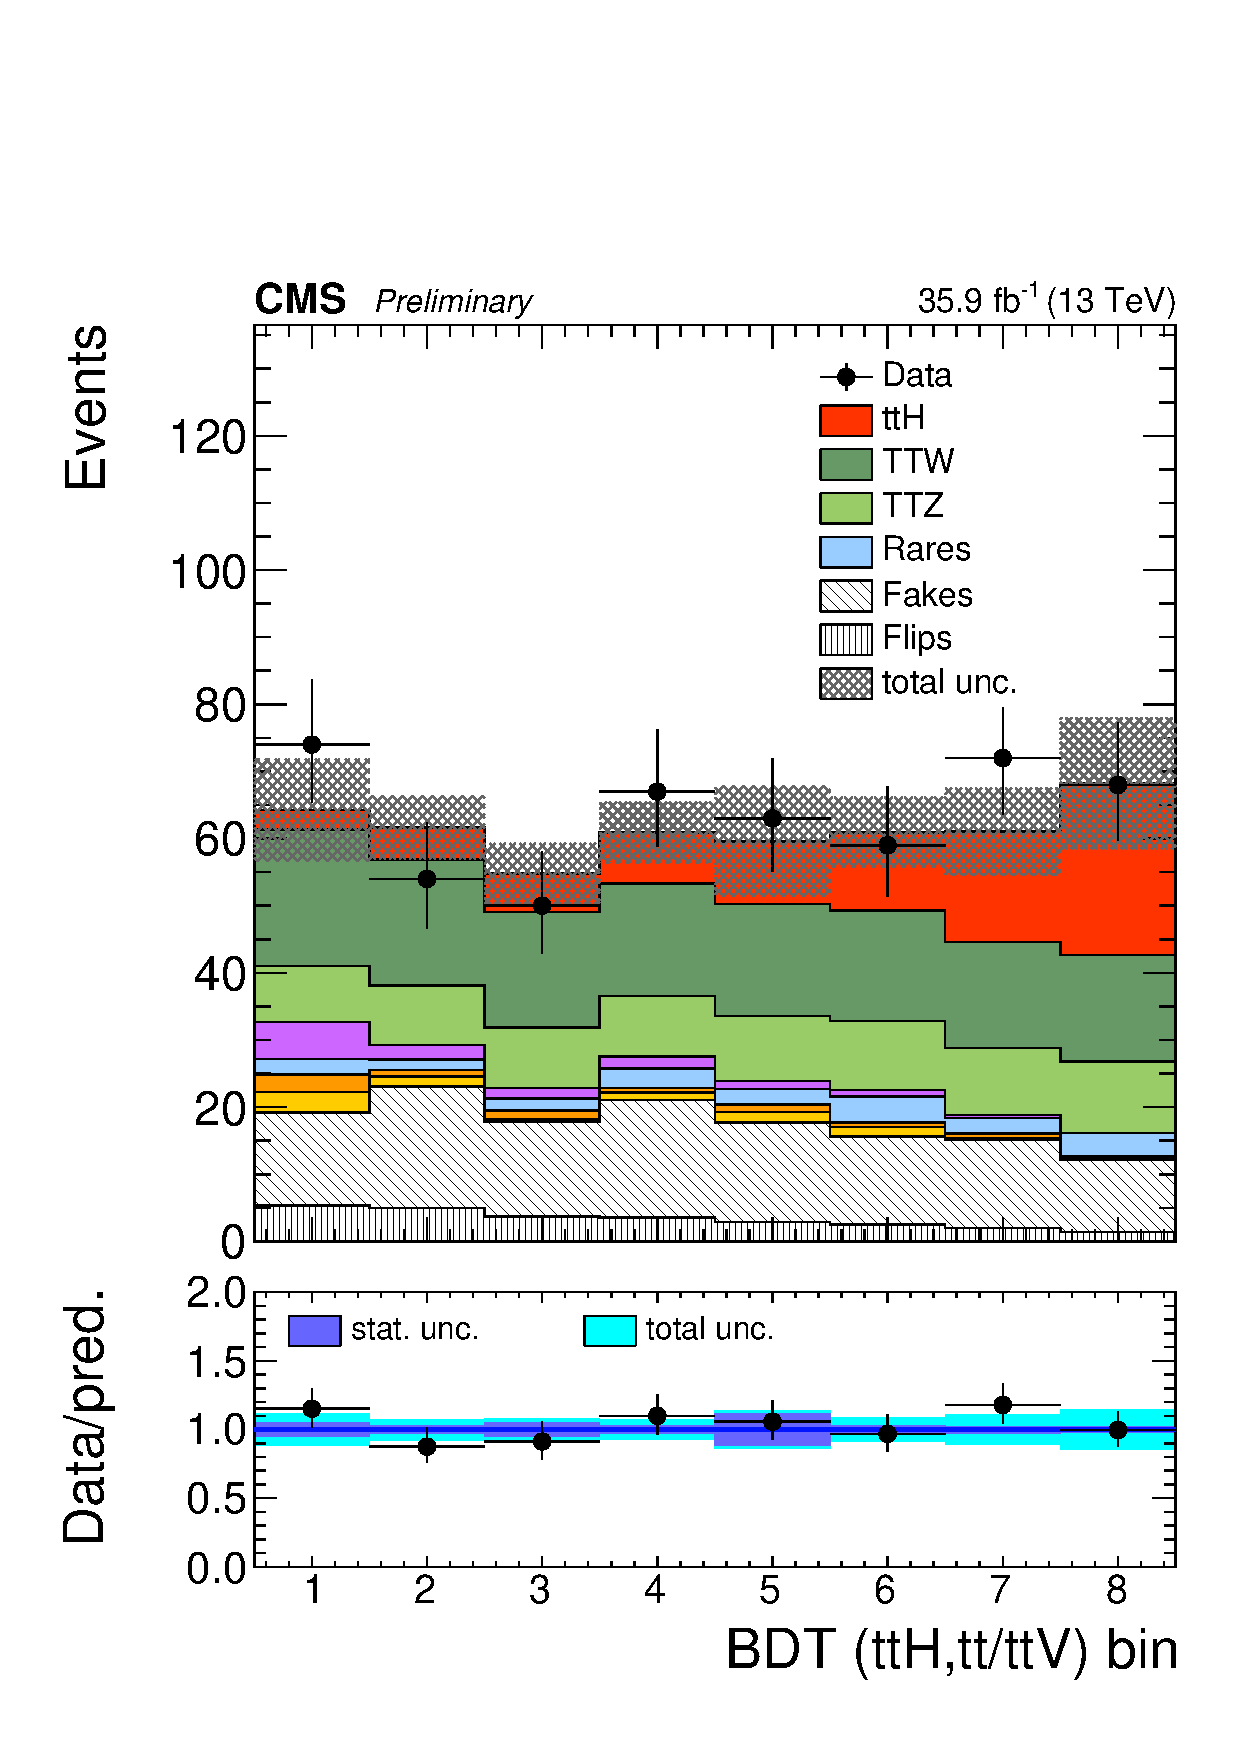
\includegraphics[width=0.32\linewidth]{plots_postfit/kinMVA_2lss_bins8_withBDTv8_withHj_ourBinning.pdf}
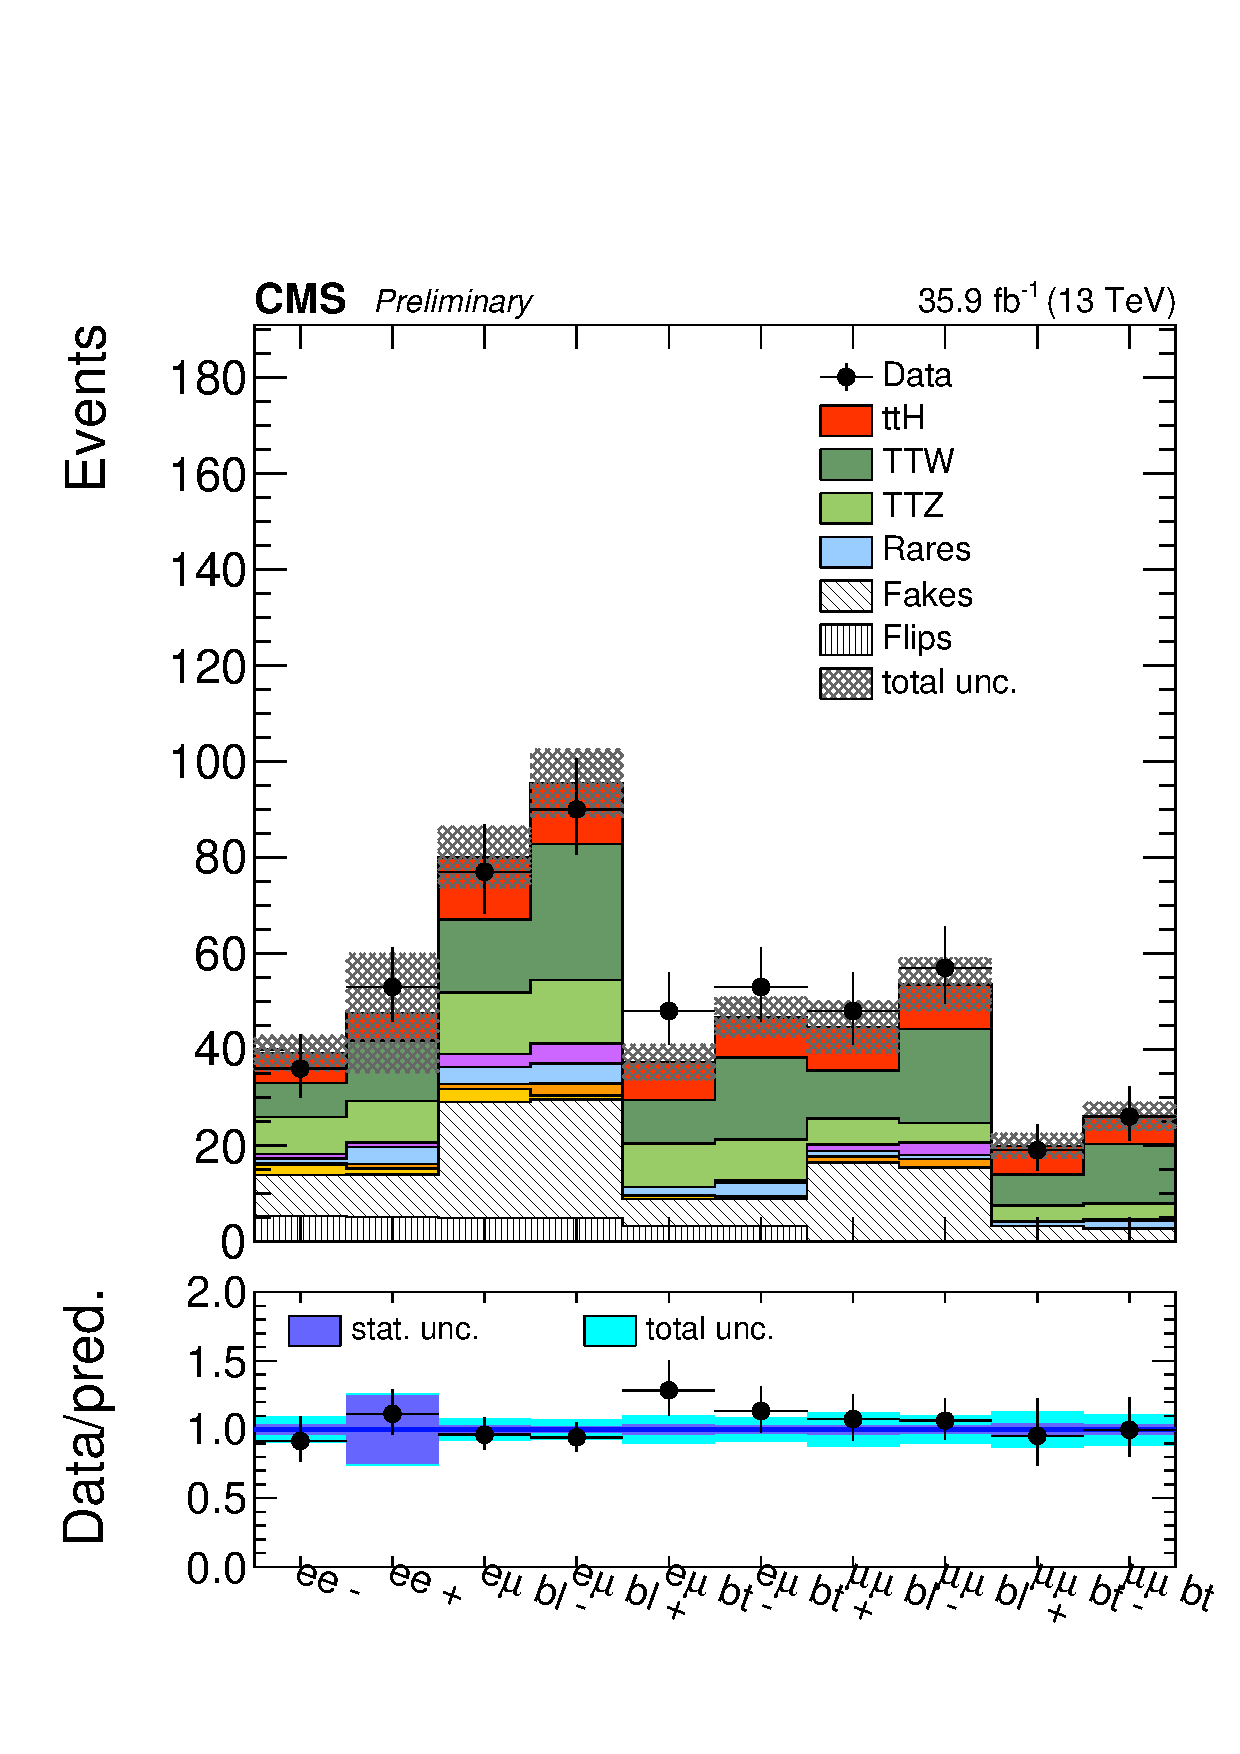
\includegraphics[width=0.32\linewidth]{plots_postfit/2lep_catIndex.pdf}\\
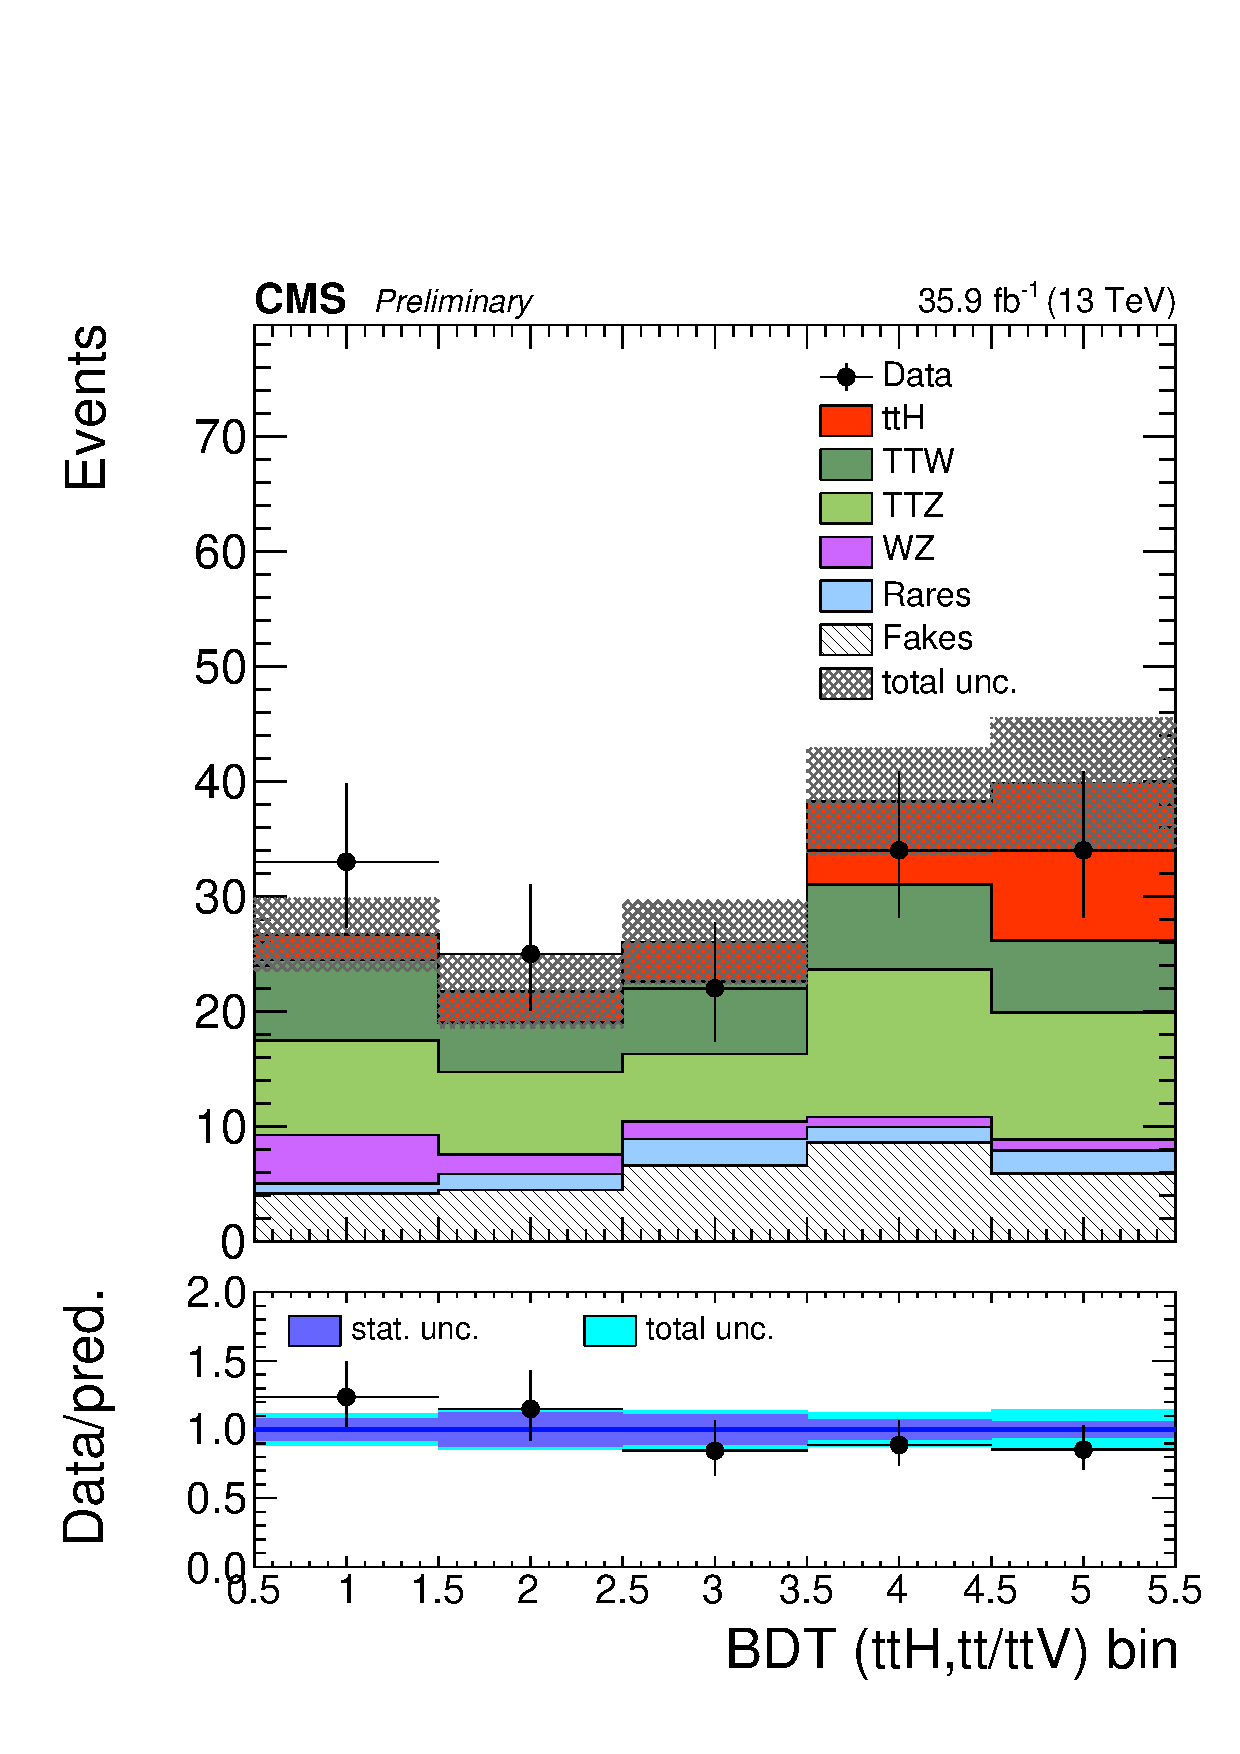
\includegraphics[width=0.32\linewidth]{plots_postfit/kinMVA_3l_bins5_withMEM_ourBinning.pdf}
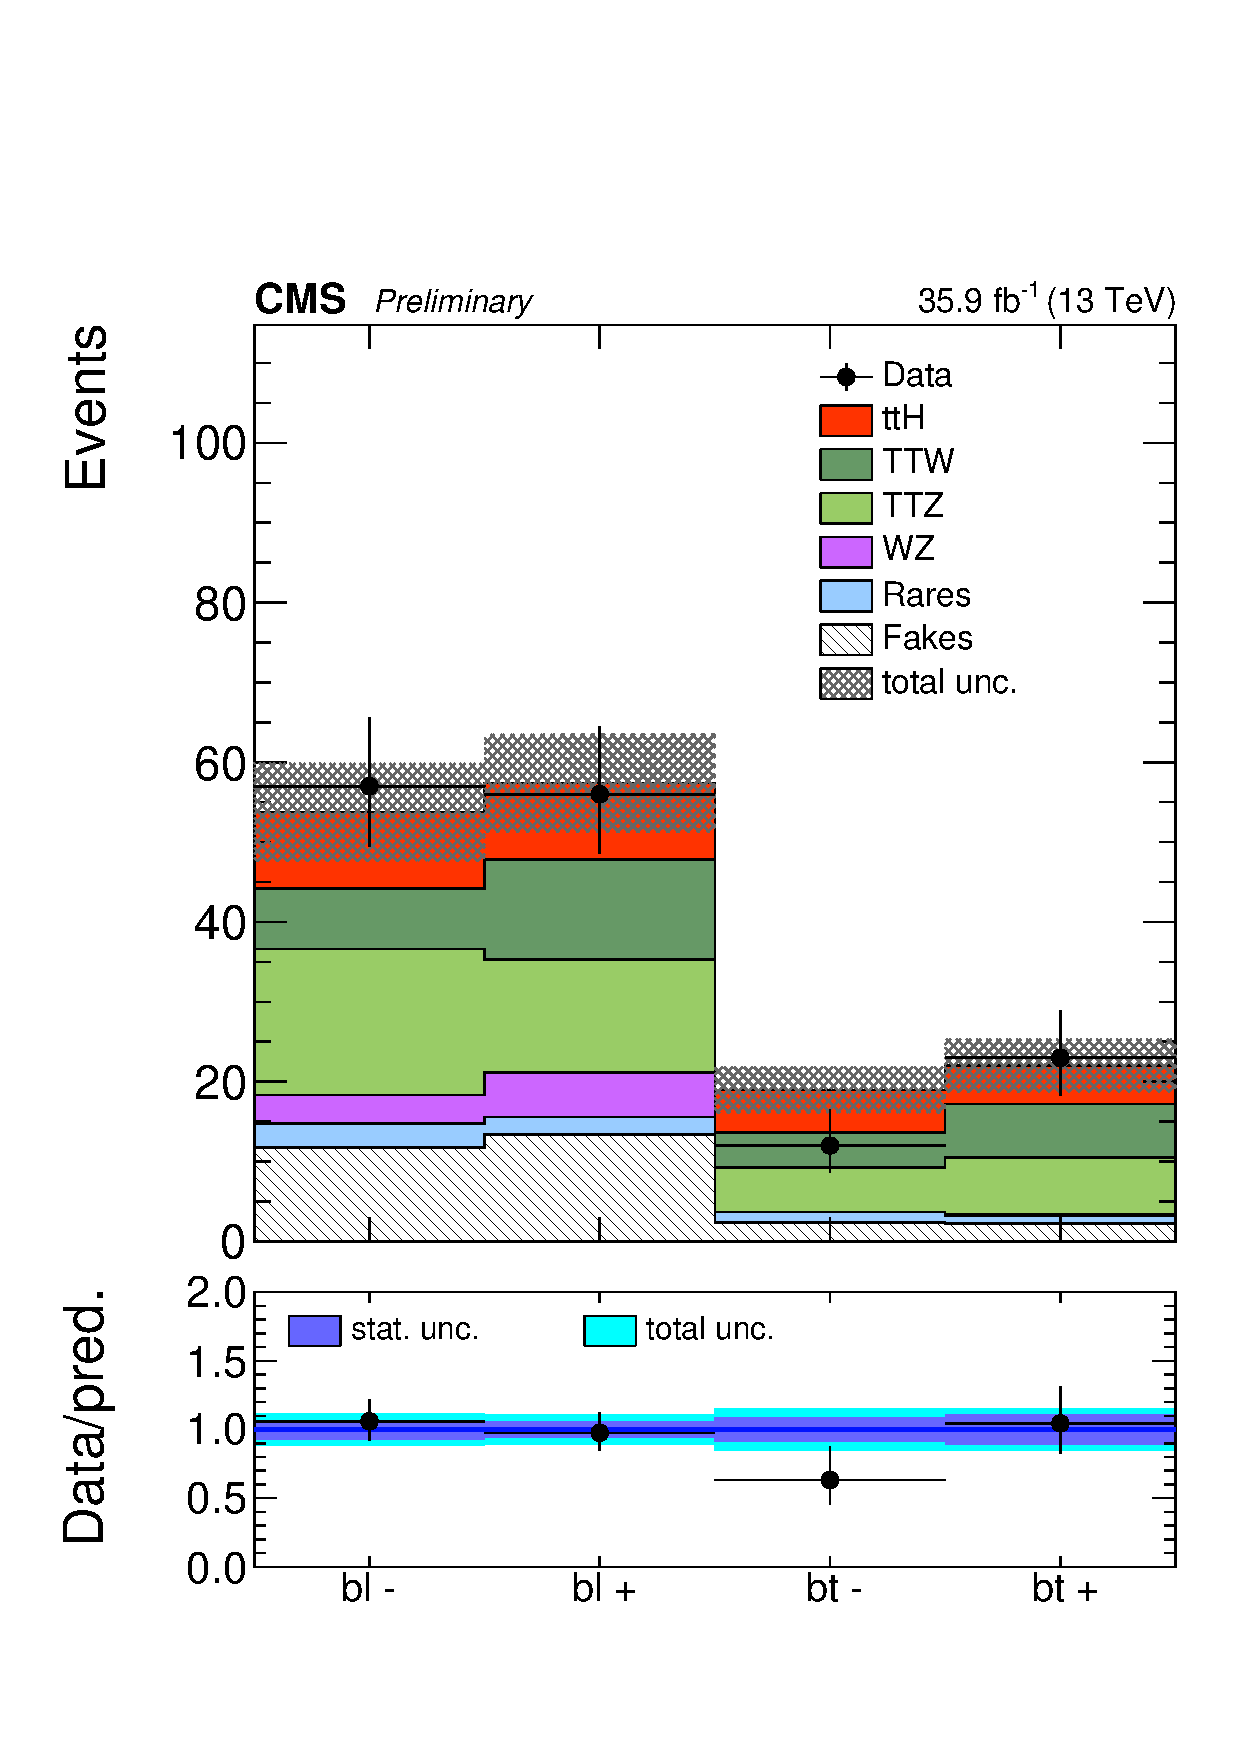
\includegraphics[width=0.32\linewidth]{plots_postfit/3lep_catIndex.pdf}
\caption{Post-fit distributions of discriminating variables and category population for 2lss (top row) and 3l (bottom row)}
\label{fig:postfit_distr}
\end{figure}


Figure~\ref{fig:impacts} shows the post-fit values of the nuisances and their correlation with the fitted signal strength.

\begin{figure}[!htb]
\centering
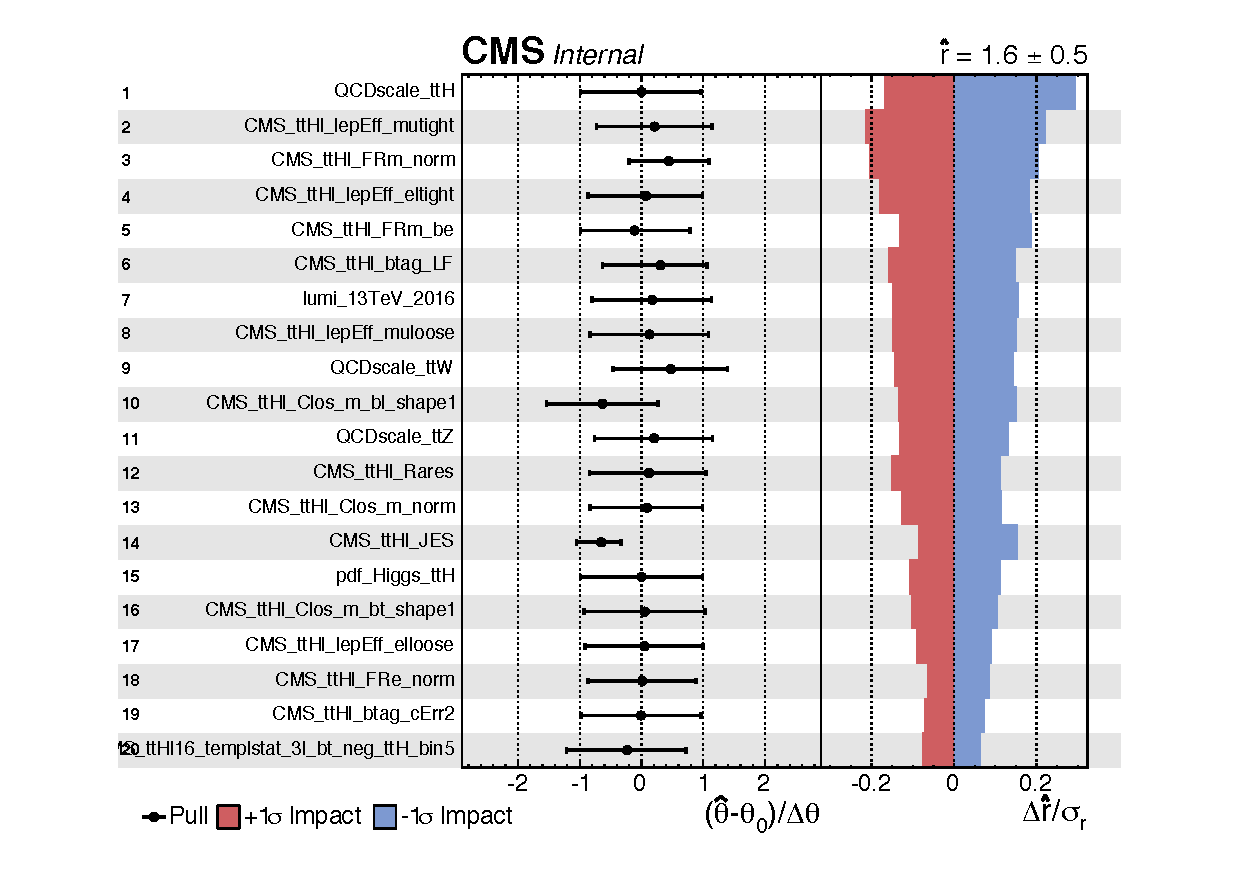
\includegraphics[width=0.80\linewidth]{plots_postfit/impacts1.pdf}\\
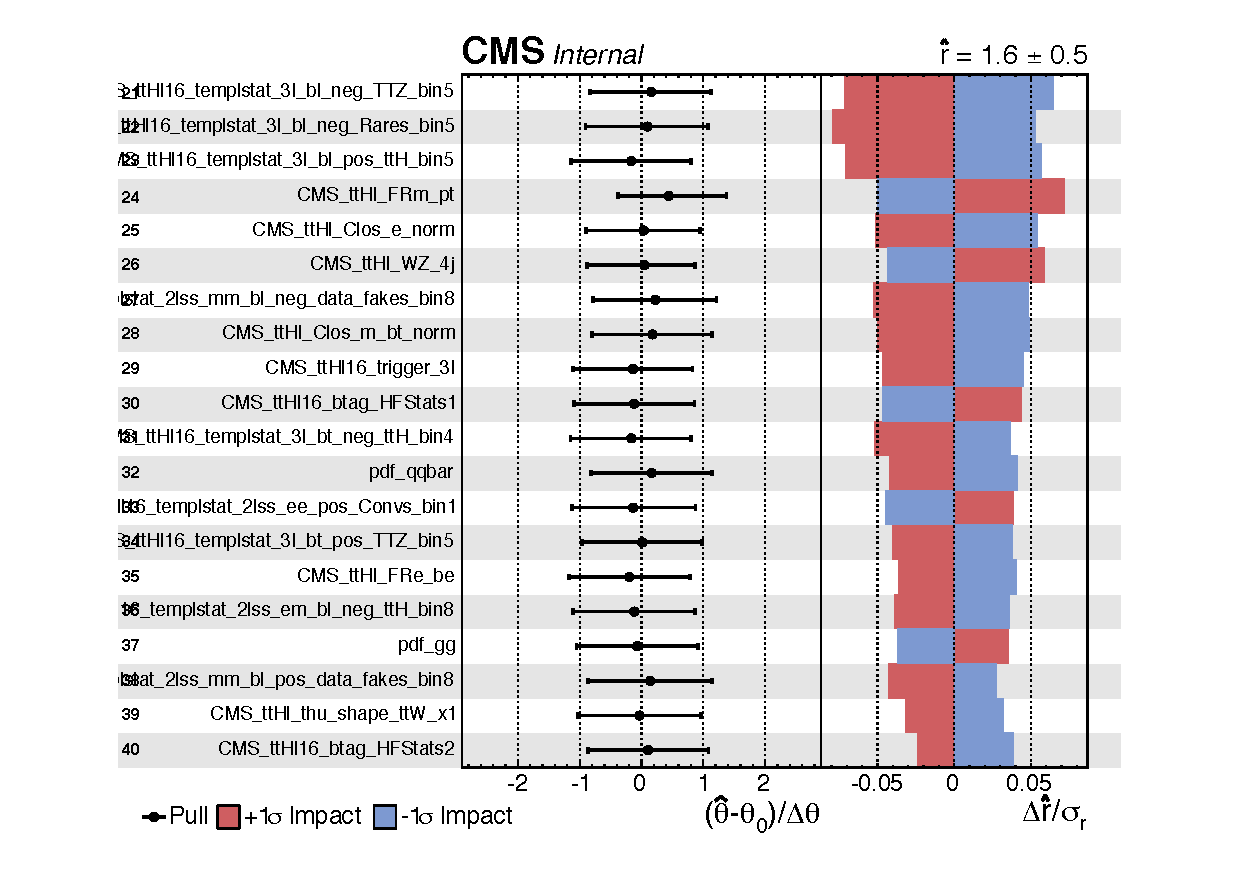
\includegraphics[width=0.80\linewidth]{plots_postfit/impacts2.pdf}
\caption{Impact plot showing the correlation between the main nuisance parameters and the best fit signal strength.}
\label{fig:impacts}
\end{figure}
